\chapter{Introduzione all'Internet of Things}
\label{chap:introduzione}
Il panorama mondiale ha, nell'ultimo decennio, riposto particolare attenzione ed interesse verso le emergenti tecnologie nel campo dell'Internet of Things (IoT). \\ Questo perchè, il paradigma IoT consente oggi di realizzare la vision ed il concept che era già stato supposto e predetto come sviluppo della rete Internet. Ovvero adempiere allo scopo di collegare il mondo (\autoref{fig:iot}). \\
Infatti, se grazie ad Interent è stato possibile collegare le persone, metterle in relazione, fornire ad essi gli strumenti per interagire tra loro, indipendentemente dalla loro posizione geografica o razza o sesso o colore, allo stesso modo, il naturale sviluppo di Internet non può che essere quello di mettere in relazione le cose. I dispositivi che siamo abituati ad utilizzare ogni giorno e che, seppur diversi ed eterogenei tra loro in termini di funzionalità, costo e posizione geografica, sono in grado di comunicare tra loro, scambiarsi dati ed informazioni al fine di cambiare definitivamente il nostro modo di lavorare, acquistare, consumare e quindi di vivere.
\begin{figure}
\begin{center}
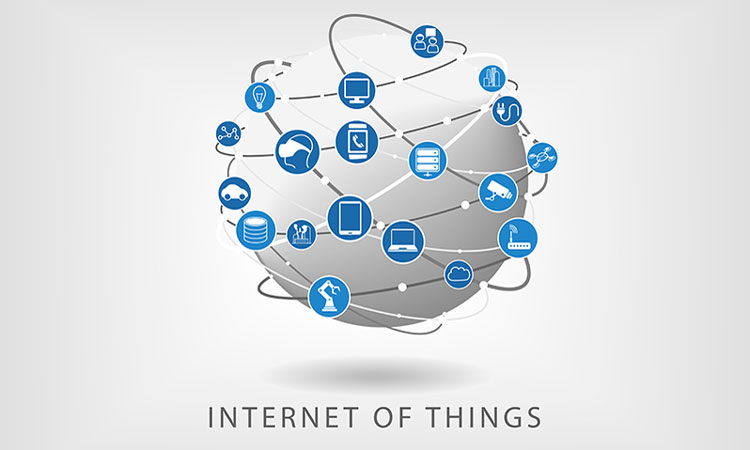
\includegraphics[width=0.7\columnwidth]{images/iot.jpg}
\end{center}
\caption{Overview del paradigma IoT}
\label{fig:iot}
\end{figure}
\\Per rendere ancora più evidente il livello innovativo introdotto dal paradigma IoT, è necessario prima effettuare una chiara distinzione tra Internet ed il World Wide Web, spesso confusi.
Con il termine Internet ci si riferisce al livello fisico dello stack protocollare realizzato da switch, routers e altri strumenti che consentono lo scambio di dati da un punto ad un altro.
Per World Wide Web si intende piuttosto un livello applicativo dello stack protocollare situato al di sopra di Internet, con il ruolo di definire una interfaccia o uno standard che renda comprensibile World Wide le informazioni trasmesse attraverso Internet.\\
Questo per evidenziare il fatto che Internet, come noi oggi lo conosciamo ed utilizziamo sia pressochè la stessa tecnologia prototipata ed utilizzata per scopi scientifico/militari nel 1969 dal DARPA denominata ARPANET (Advanced Research Projects Agency NETwork) dalla quale, nel 1983 naque Internet.\\
Il paradigma IoT si propone quindi come la prima, vera, evoluzione di Internet con la potenzialità di cambiare radicalmente il modo di vivere, imparare e lavorare. \cite{famous:paper_cisco_intro}
\begin{figure}
	\begin{center}
		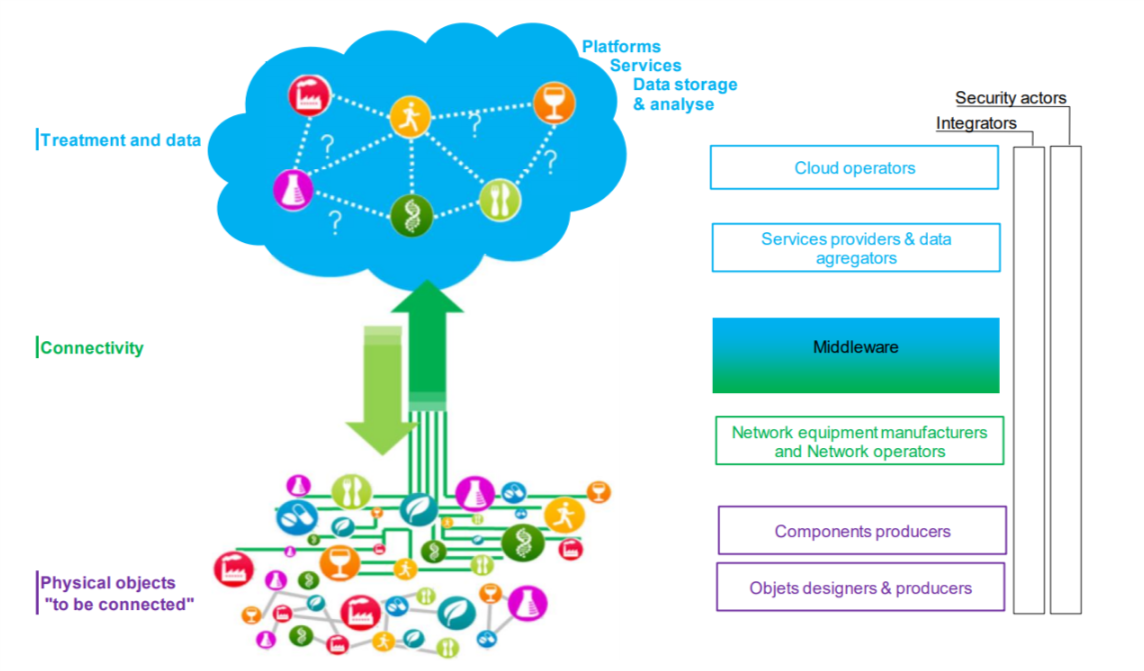
\includegraphics[width=0.9\columnwidth]{images/iot_revolution.png}
	\end{center}
	\caption{Gli oggetti collegati ad Internet possono essere progettati per una grande varietà di applicazioni \cite{famous:paper_francese}}
	\label{fig:iot_revolution}
\end{figure}




\section{I Numeri dell'IoT}
\label{sec:i_numeri_dell_iot}
Alla luce di quanto detto, si può quindi riassumere il significato del termine Internet of Things come la connessione di un numero crescente di dispositivi ed oggetti che comunicano tra di loro sfruttando la rete Internet. \cite{famous:paper_full_intro}\\
Ci si aspetta, ed i numeri attuali lo dimostrano, che il mondo dell'IoT abbia una crescita esponenziale, connettendo miliardi di dispositivi in un tempo relativamente breve. Questo, ovviamente non può che avere un enorme impatto dal punto di vista tecnologico ed economico.\\
Dal punto di vista \textbf{tecnologico}, va affrontata la sfida di creare delle infrastrutture scalabili che possano supportare il numero crescente di dispositivi e la crescente mole di dati tra di essi trasmessa. 
\begin{figure}
	\begin{center}
		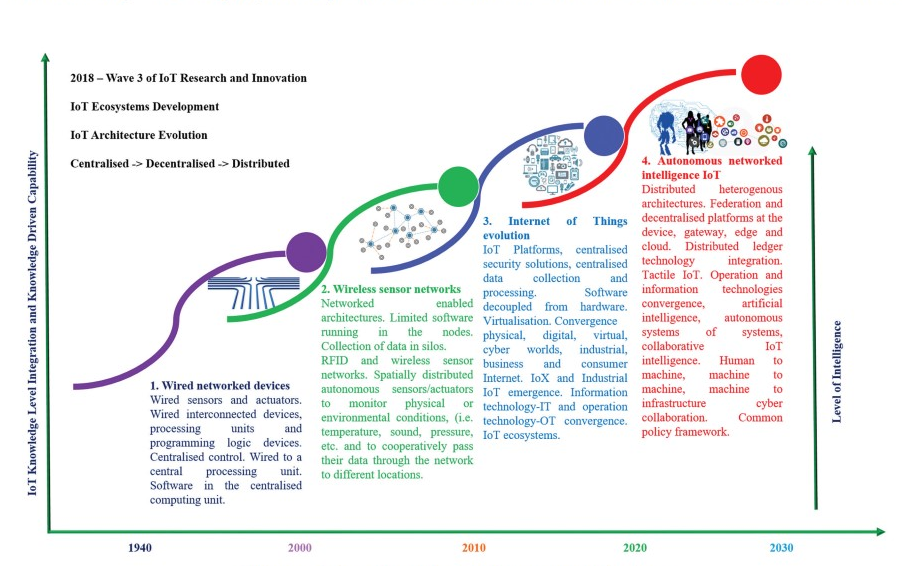
\includegraphics[width=0.7\columnwidth]{images/iot_tech_data.png}
	\end{center}
	\caption{Number of IoT devices roadmap}
	\label{fig:iot_tech_data}
\end{figure}
Va inoltre notato come tali stime non tengano in conto anche dei vantaggi di una rapida ascesa di Internet ma che si basino solo sui dati noti al momento della stima.\\
La sfida tecnologica è dovuta al fatto che Internet è una tecnologia che risale allo scorso secolo che non fosse stata progettata per supportare un così crescente numero di dispositivi connessi alla rete.\\
Internet, infatti, fa largo uso del protocollo IP per la assegnazione di indirizzi pubblici univoci a ciascun device (o meglio connessione fisica alla rete) . Nella sua versione IPv4, ciascun indirizzo è formato da 32 bit, limitando così il numero massimo di indirizzi univoci a:
\begin{equation}
2^{32} = 4.294.967.296 \cong 4,3 \cdot 10^9
\end{equation}
Ma va tenuto presente che non tutti sono utilizzabili in quanto alcuni di questi siano riservati per specifici utilizzi.
Tale protoccolo quindi poco si adatta alla frenetica crescita del numero di dispositivo collegati ad Internet, motivo per il quale, già nel 1998 viene proposta una nuova versione di questo protocollo denominata IPv6 che sarà analizzata in dettaglio nella \autoref{sec:iot_enabling_technologies}. Il primo, evidente vantaggio di questa nuova versione, sta nel fatto che IPv6 riserva 128 bit per la codifica di ciascun indirizzo, portando così il numero massimo di indirizzi univoci assegnabili a \cite{book:ref_book_1}:
\begin{equation}
2^{128} \cong 3,4 \cdot 10^{38}
\end{equation}
Questo inevitabile sviluppo del protocollo IP è completamente giustificato dalle stime sulla rapida crescita del numero di oggetti che vengono connessi alla rete Internet.\\
\begin{figure}
	\begin{center}
		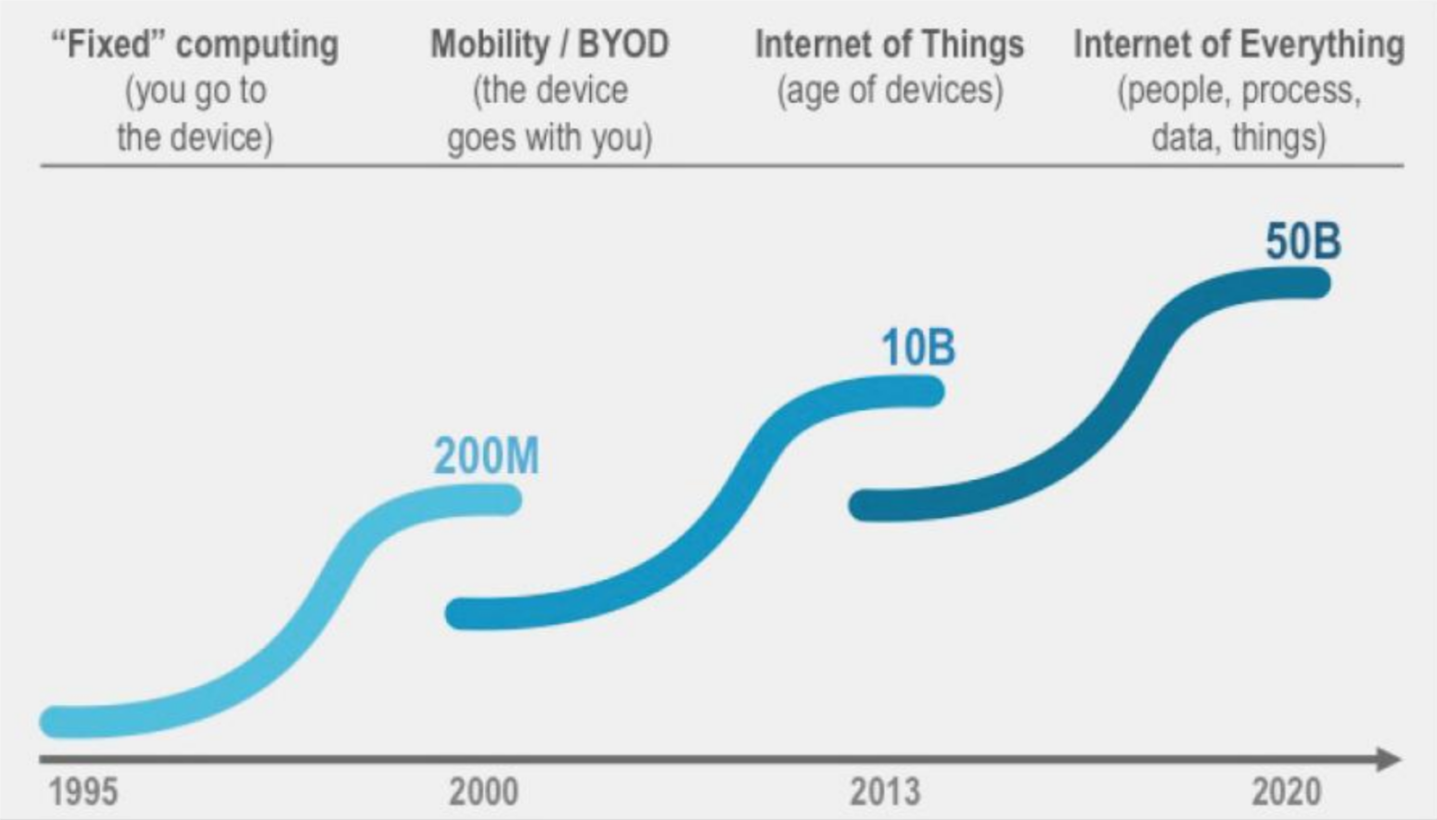
\includegraphics[width=0.9\columnwidth]{images/numbers_devices.png}
	\end{center}
	\caption{Previsioni della rapida crescita sul numero di oggetti connessi ad Internet \cite{famous:paper_cisco_2013}}
	\label{fig:numbers_devices}
\end{figure}
Dal punto di vista \textbf{economico}, una simile ascesa del numero di dispositivi connessi in rete, in un campo così ampio di applicazione, ha un tale impatto da giustificare gli investimenti su infrastrutture di telecomunicazione e sui plant industriali. 
\begin{figure}
	\begin{center}
		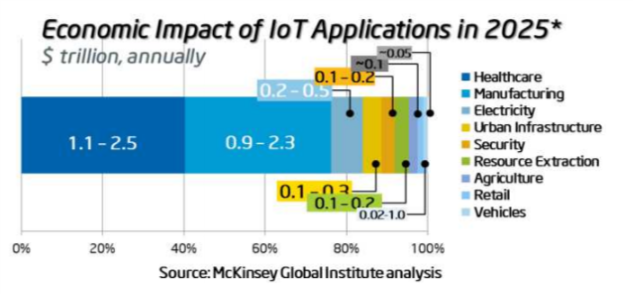
\includegraphics[width=0.9\columnwidth]{images/numbers_economic.png}
	\end{center}
	\caption{Impatto economico di applicazioni IoT nel 2025 fornito dal McKinsey Global Institute \cite{famous:mck}}
	\label{fig:numbers_economic}
\end{figure}
\begin{figure}
	\begin{center}
		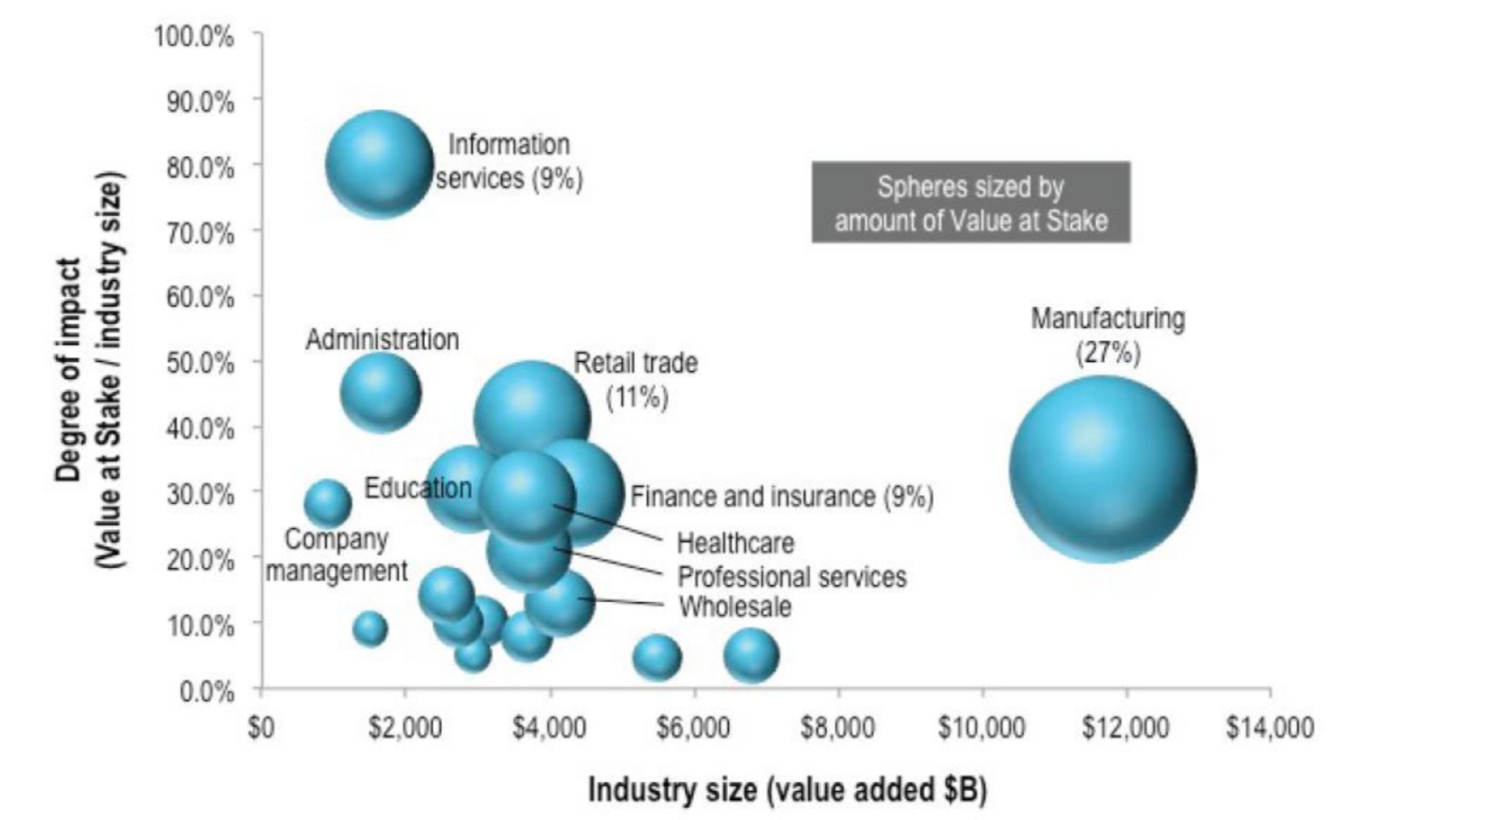
\includegraphics[width=0.9\columnwidth]{images/numbers_where.png}
	\end{center}
	\caption{Campi di applicazione nei quali si stima il maggiore sviluppo reso possibile dall'IoT \cite{famous:paper_cisco_2013}}
	\label{fig:numbers_where}
\end{figure}
Un simile andamento del mercato legato al mondo IoT è stato descritto anche in \cite{famous:paper_indian_market} dove si evidenzia come l'andamento del mercato globale, fortemente influenzato dal crescente numero di dispositivi connessi alla rete, possa attrarre una grossa percentuale di investitori e di valore economico aggiunto per le imprese.

\begin{table}
	\begin{center}
	\begin{tabular}{|c|m{8cm}|}
		\hline
		\textbf{S.N.} & \textbf{IoT Global} \\
		\hline
		1. & Il mercato IoT crescerà da 15.4 miliardi di dispositivi nel 2015 a 30.7 miliardi di dispositivi nel 2020 e 75.4 miliardi nel 2025 \\
		\hline
		2. & Nel periodo 2016-2021, le spese globali su prodotti e servizi legati al mondo IoT raggiungeranno i \$120-\$253 miliardi attraendo il 16\% CAGR \\
		\hline
		3. & IoT crescerà da \$10 a \$15 trilioni di GDP globale nei prossimi 20 anni \\
		\hline
		4. & Nel 2020 la guida autonoma e dispositivi IoT cresceranno globalmente \\
		\hline
	\end{tabular}
\caption{Previsione dell'andamento globale del mercato di prodotti e servizi legati al mondo IoT \cite{famous:paper_indian_market}}
\label{tabel:market_global}
\end{center}
\end{table}






\section{IoT Enabling Technologies}
\label{sec:iot_enabling_technologies}
L'idea di una rete Internet che consentisse la comunicazione a livello globale tra persone o tra persone e cose o tra cose era già da molto tempo una visione condivsa di quello che sarebbe potuto essere lo sviluppo di Internet. \\
Tale visione è oggi possibile grazie alla diffusione capillare in qualsiasi strumento di piccoli, economici e potenti dispositivi di calcolo. \\
Tuttavia, affinchè una simile rivoluzione tecnologia si paventasse, era necessario superare i tradizionali protocolli di comunicazione tipici della rete Internet (IPv4, HTTP) e creare conseguentemente delle nuove tecnologie per la comunicazione che fossero ottimizzate per le nuove esigenze (IPv6, MQTT, CoAP, etc.).
Va infatti ricordato ancora una volta che la vision dell'IoT sia quella di abilitare una comunicazione tra qualsiasi tipo di dispositivo che abbia al suo interno una unità di calcolo. Questo significa stabilire una comunicazione tra dispositivi eterogenei, dispositivi che assolvono diversi compiti ed adempiono a diverse necessità e che sono molto spesso anche dotati di una diversa e limitata potenza di elaborazione. \\
Di qui la necessità di nuovi protocolli e tecnologie di comunicazione che non solo garantissero la trasmissione sicura di una grossa mole di dati tra un grande numero di dispositivi, ma che fossero anche dei protocolli leggeri dal punto di vista computazionale ed ovviamente economici, così da poter essere integrati in qualsiasi dispositivo, da quelli destinati all'industria a quelli destinati al mercato consumer.\\
\begin{table}
	\begin{center}
		\begin{tabular}{|c|m{8cm}|}
			\hline
			\textbf{Tipologia di Comunicazione} & \textbf{Descrizione} \\
			\hline
			M2M & Machine to Machine comunication. Una macchina comunica con un'altra macchina per accumulare informazioni e scambiare dati.  \\
			\hline
			H2H & Human to Human comunication. Comunicazione tra uomini mediante gesti o mediante il linguaggio \\
			\hline
			D2D & Device to Device comunication. Comunicazioe tra due dispositivi che eviti infrastrutture di routing della comunicazione intermedie. Ciascun dispositivo comunica direttamente con un altro dispositivo che sia da esso direttamente raggiungibile senza intermediari \\
			\hline
		\end{tabular}
		\caption{Le metodologie di comunicazione \cite{famous:paper_communication_metodology}}
		\label{tabel:comunication_metodology}
	\end{center}
\end{table}
Data la complessità della sfida tecnologica da fronteggiare e considerata l'eterogeneità del problema e delle necessità nei diversi campi applicativi,
sono stati sviluppate e proposte diverse tipologie di tecnologie e protocolli di comunicazione. \\

\subsection{Il Protocollo IPv6}
Come già anticipato nella \autoref{sec:i_numeri_dell_iot}, il primo enabler necessario per l'avvento dell'Internet of Things è proprio quello che garantisca che ogni dispositivo, oggetto, sensore o persona possa connettersi alla rete Internet e scambiare dati con altri dispositivi. Per far si che questo sia possibile, è quindi necessario dotare ciascun dispositivo di un indirizzo che identifichi univocamente quell'oggetto nella rete Internet. Questo compito, attualmente, è affidato perlopiù al protocollo IPv4 che identifica un elemento in rete attraverso un indirizzo IP pubblico univoco composto da 32 bit.\\ Visto il limitato numero di indirizzi IP che il protocollo IPv4 è in grado di fornire (alcuni dei quali non utilizzabili), già nel passato, si sono dovuti apportare alcuni accorgimenti e modifiche al protocollo. 
Già negli anni ottanta, infatti, si è giunti ad una saturazione di IPv4 che non era più in grado di adempiere al suo compito di fornire un indirizzo univoco, vista la crescita esponenziale avuta dalle reti LAN.
A tal scopo, sono state escogitate altre tecniche (come il mascheramento) per continuare ad utilizzare il vecchio protocollo IPv4 nonostante la sua limitata capacità.\\
Sebbene queste tecniche ci abbiano consentito e ci stanno consentendo di continuare ad utilizzare il protocollo IPv4, nonostante la capillare espansione della rete Internet, quando si parla di Internet of Things o addirittura di Internet of Everything, questi stratagemmi non sono più sufficienti.
Dalle stime sulla crescita esponenziale del numero di oggetti connessi ad Internet, si intuisce subito che sia necessaria una evoluzione del protocollo IPv4 già proposta nel 1998, ovvero il protocollo IPv6.
\begin{figure}
	\begin{center}
		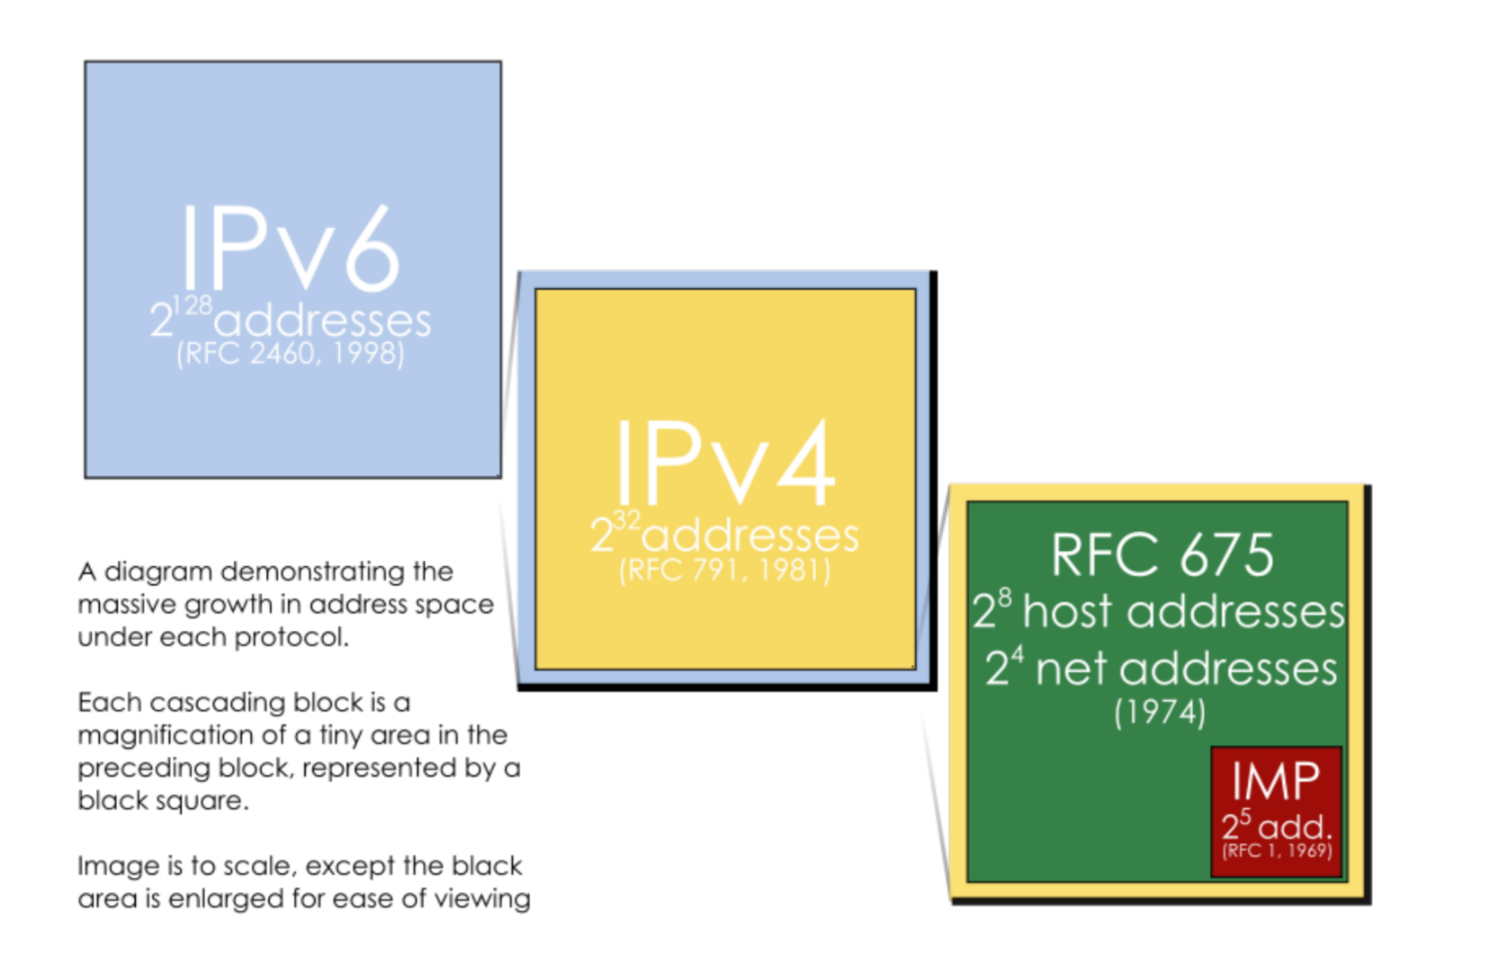
\includegraphics[width=0.9\columnwidth]{images/slide_ipv4_ipv6.png}
	\end{center}
	\caption{Evoluzione dello spazio destinato all'indirizzamento \cite{book:slide_Grieco}}
	\label{fig:slide_ipv4_ipv6}
\end{figure}
Conseguentemente ad una modifica alla dimensione dello spazio di indirizzamento, è avvenuta anche una modifica per quanto riguarda l'header di un pacchetto trasmesso attraverso Internet in formato IPv6.
\begin{figure}
	\begin{center}
		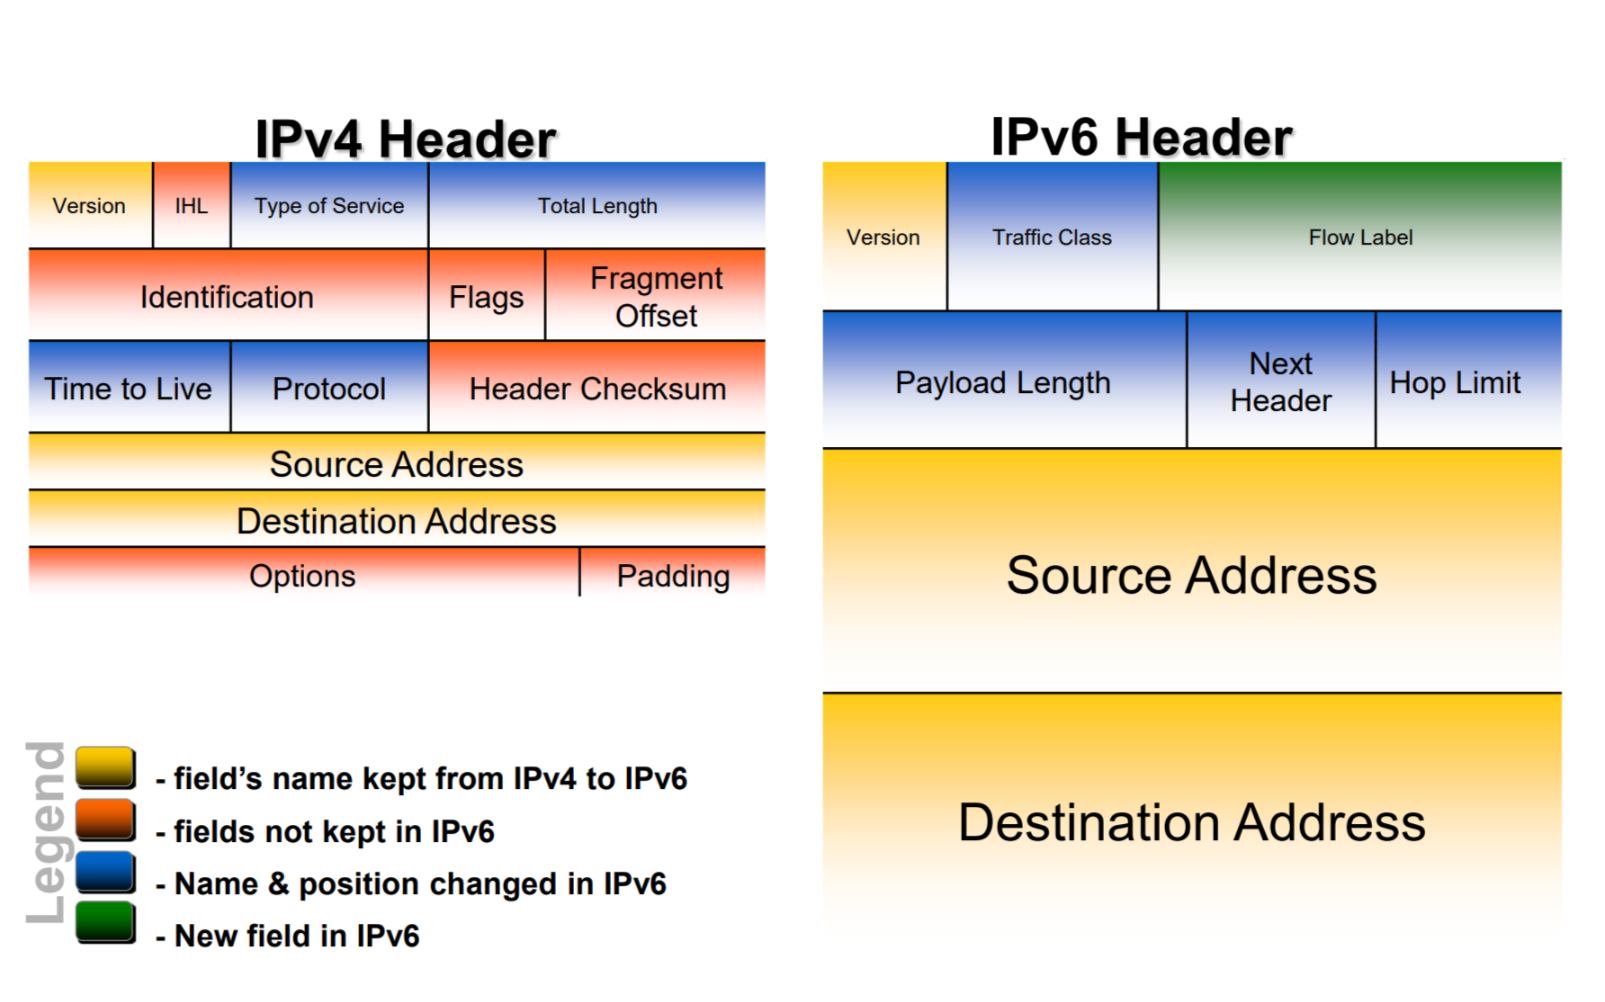
\includegraphics[width=0.9\columnwidth]{images/slide_header_ipv4_ipv6.png}
	\end{center}
	\caption{Confronto tra l'header nei protocolli IPv4 ed IPv6 \cite{book:slide_Grieco}}
	\label{fig:slide_header_ipv4_ipv6}
\end{figure}
\\Tra le principali caratteristiche del protocollo IPv6 rispetto all'IPv4 ci sono: \cite{book:slide_Grieco} \cite{book:ref_book_1}
\begin{itemize}
	\item Spazio di indirizzamento più grande (128 bit)
	\item Nuovo formato dell'header che minimizza l'overhead
	\item Infrastruttura di routing e schema di indirizzamento progettati appositamente per essere efficienti e gerarchici
	\item Supporto built-in per la sicurezza (IPSec) \cite{famous:paper_ipsec}
	\item Supporto per la QoS garantita da nuovi campi nell'header
\end{itemize}
I vantaggi di un protocollo (IPv6) progettato appositamente per soddisfare le nuove richieste della rete Internet sono subito evidenti:
\begin{itemize}
	\item[\checkmark] Maggiore disponibilità di indirizzi IP univoci
	\item[\checkmark] Numero inferiore di campi all'interno dell'header
	\item[\checkmark] Minore capacità computazione richiesta per la lettura dell'header
\end{itemize}

\subsection{Molte applicazioni, diversi protocolli}
Così come il protocollo IP diviene obsoleto con l'avvento dell'era dell'Internet of Things, rendendo necessario un upgrade a nuovi standard (IPv6), anche le infrastrutture di rete ed i protocolli di più basso livello lo diventano.
Al fine di rendere possibile la connessione persistente ed onnipresente richiesta da molte delle applicazioni IoT, è necessario che siano aggiunte molte più features e funzionalità alle attuali tecnologie a banda larga.
Le evoluzioni del 4G e le emergenti reti 5G saranno pertanto caratterizzate dall'interoperabilità e dall'integrazione tra più reti di accesso radio. \cite{famous:paper_Grieco_1}\\
Tuttavia, considerato il grande campo di applicazione ed il grande numero di dispositivi legati al mondo dell'IoT, sarebbe riduttivo limitare i protocolli di comunicazione di basso livello alle sole evoluzioni del 4G e del 5G. Una grande varietà di tecnologie di comunicazione, infatti, ha preso piede, rispecchiando così la grande varietà di domini applicativi, dispositivi e requirements legati all'IoT.
Tra le più rilevanti nel campo della comunicazione domestica o locale emergono Bluetooth Low Energy \cite{famous:paper_1} and Zigbee \cite{famous:paper_2}. Mentre altri protocolli come WiFi, LowPower Wide Area Networks (LPWA) \cite{famous:paper_3} e le comunicazioni cellulari come 3GPP , 4G o 5G \cite{famous:paper_Grieco_1} hanno uno scope più ampio, abilitando la comunicazione tra dispositivi anche molto distanti tra loro.\\
Tutti questi protocolli di comunicazione e le infrastrutture che li supportano, condividono alcune caratteristiche che sono comunemente necessarie a tutti gli oggetti connessi in rete:
\begin{itemize}
	\item Scalabilità
	\item Bassa capacità computazionale richiesta
	\item Economicità
	\item Bassi consumi energetici
	\item Supporto dell'ecosistema IP
\end{itemize}

\subsection{L'Application Layer per i dispositivi IoT}
A valle di tutte le considerazioni effettuate sugli enablers necessari al mondo dell'Internet of Things per instaurare una comunicazione a basso livello tra oggetti, è bene anche considerare che, al pari dei protocolli e tecnologie di basso livello, anche i protocolli di comunicazione di alto livello (application layer) diventano obsoleti ed inadatti all'IoT.\\
Uno dei principali motivi per i quali Internet come lo conosciamo ed utilizziamo oggi ha avuto un capillare sviluppo a livello globale ed ha consentito la massiccia nascita di applicazioni e servizi ad esso legati, è certamente dovuto al World Wide Web. Come già anticipato, infatti, la rete Internet nata per scopi militari/scientifici, ha come unico obiettivo quello di trasmettere una informazione, da un punto ad un altro, anche molto distanti.
Tuttavia, che cosa venga trasmesso attraverso Internet, cioè quali dati e cosa essi significhino e come sono codificati, è fuori dallo scope di Internet. In riferimento alla \autoref{fig:application_layer_stack}, questi compiti sono svolti da livelli superiori allo stack protocollare TCP-IP che si occuperanno di codificare determinate informazioni o dati, passarli ad i livelli inferiori (Internet) e poi trasmetterli.
\begin{figure}
	\begin{center}
		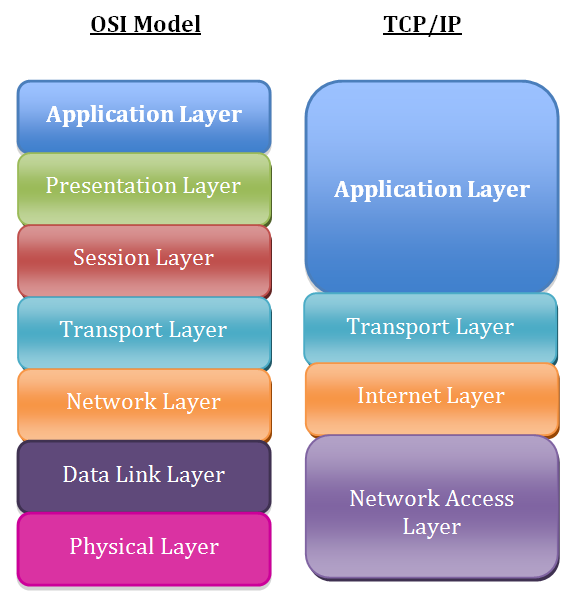
\includegraphics[width=0.6\columnwidth]{images/application_layer_stack.png}
	\end{center}
	\caption{Modello TCP-IP (destra) in confronto con il modello ISO-OSI (sinistra) \cite{book:wikipedia}}
	\label{fig:application_layer_stack}
\end{figure}
Alla base del World Wide Web e quindi del comune utilizzo di Internet è presente il protocollo HTTP o HTTPS. Questo protocollo appartiene all' Application Layer di \autoref{fig:application_layer_stack} ed è utilizzato come principale sistema per la trasmissione di informazioni sul Web attraverso una architettura Client-Server che, a livello più basso (Transport Layer) utilizza il protocollo TCP.
Questo protocollo, unitamente ad HTML, URIs e REST, hanno portato all'enorme successo del World Wide Web. \cite{book:slide_Grieco}
Per quanto il protocollo HTTP sia oggi diffuso ed utilizzato e si potrebbe esportare anche nei dispositivi legati al mondo dell'Internet of Things, vanno considerati alcuni svantaggi e limitazioni al suo utilizzo.
\begin{itemize}
	\item[$\times$] HTTP utilizza a livello di trasporto il protocollo TCP il quale risulterebbe troppo pesante
	\item[$\times$] HTTP utilizza i protocolli SSL/TLS per garantire elevati standard di sicurezza i quali risulterebbero troppo pesanti
\end{itemize}
\begin{figure}%
	\centering
	\subfloat[Raspberry Pi 3]{{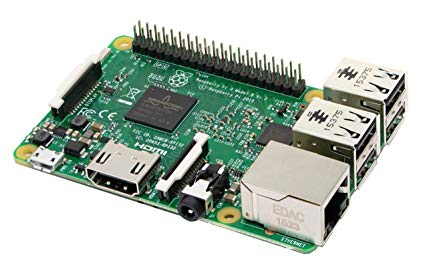
\includegraphics[width=5cm]{images/application_layer_raspberry} }}%
	\qquad
	\subfloat[Texas Instruments Zigbee Development Kit]{{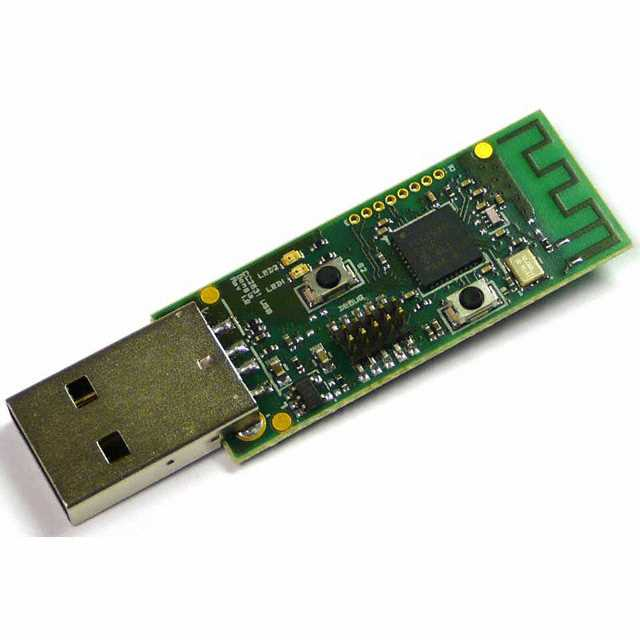
\includegraphics[width=5cm]{images/application_layer_device} }}%
	\caption{Dispositivi con limitate capacità computazionali, RAM e ROM}%
	\label{fig:application_layer_devices}%
\end{figure}
A livello applicativo vengono pertanto progettati dei nuovi protocolli che risultino più leggeri nell'elaborazione in dispositivi dalle capacità limitate, ma che al contempo ereditino i vantaggi, le funzionalità e la compatibilità con lo standard HTTP. Tra i più famosi CoAP, AMQP e MQTT.\\
In riferimento al prototipo sviluppato in questo lavoro di tesi, a valle delle scelte progettuali mostrate nel \autoref{chap:tre}, si è ritenuto opportuno utilizzare il protocollo MQTT per il livello applicativo e pertanto si intende adesso analizzarlo più nel dettaglio.

\subsubsection{Il Protocollo MQTT}
\label{sec:MQTT_protocol}
Per la condivisione di dati attraverso Internet, il protocollo MQTT sta diventando uno dei più popolari. Questo anche grazie al fatto che sia un protocollo leggero e che quindi bene si adatti ai sistemi ed alle necessità del mondo dell'Internet of Things, ovvero condividere una grossa mole di dati in real-time.
Il protocollo MQTT, realizzato nel 1999 da Dr. Andy Stanford-Clark e Arlen Nipper, nasce come un protocollo open source di messaggistica con architettura publish-subscribe. La sua progettazione è stata proprio pensata per funzionare in dispositivi limitati, reti inaffidabili o ad elevata latenza e che fosse anche facile da implementare. \cite{famous:paper_mqtt_intro} \cite{book:slide_Grieco}
Gli attori principali che compongono questo protocollo sono pertanto:
\begin{itemize}
	\item MQTT Broker
	\item Publisher
	\item Subscriber
\end{itemize}
Per lo scambio di dati attraverso il protocollo MQTT, è predisposto un controllore centrale che viene utilizzato per distribuire i messaggi.\\ Questo è detto \textbf{MQTT Broker} ed ha il compito di inoltrare, filtrare ed assegnare le priorità alle publish request che il broker riceve dai publisher dirette ad i subscriber. \\
I \textbf{Publisher} sono coloro che si occupano di generare i dati. Possono infatti essere sensori, generatori di dati o sistemi integrati, i quali, per comunicare attraverso MQTT, devono specificare due elementi principali: messaggio da inviare e topic. Solo in questo modo, attraverso il topic di un messaggio, il Broker potrà ricevere correttamente i messaggi dai publisher e decidere quale Subscriber debba ricevere il messaggio. \\
I \textbf{Subscriber} infine, non sono altro che dispositivi o oggetti o altri Publisher, che si sottoscrivono ad uno o più topic. Ovvero che richiedo al Broker di ricevere tutti i messaggi ad esso inviatogli che siano apparteneneti ad un certo topic.
I Subscribers possono quindi ricevere i soli messaggi che abbiano lo stesso topic (o gli stessi topic) di quello ai quali si sono sottoscritti.
\begin{figure}
	\begin{center}
		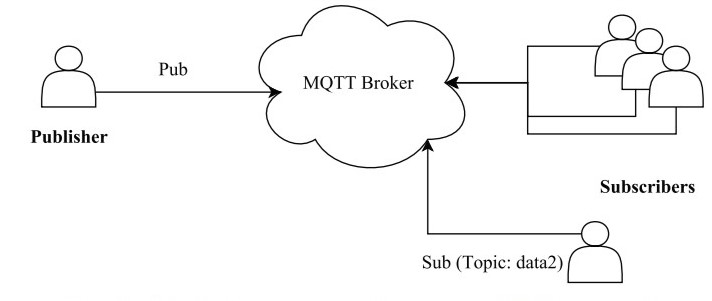
\includegraphics[width=0.6\columnwidth]{images/mqtt_schema.jpg}
	\end{center}
	\caption{Comunicazione attraverso il protocollo MQTT \cite{famous:paper_mqtt_intro}}
	\label{fig:mqtt_schema}
\end{figure}
Dalla \autoref{fig:mqtt_schema} si evince come, se il Publisher invii un messaggio al Broker caratterizzato dal topic : \textit{data2}, allora questo sarà ricevuto dal solo Subscriber in  basso, quello cioè in 'ascolto' sul topic \textit{data2}.\\
Il protocollo MQTT, infine, grazie alla sua leggerezza rispetto ad HTTP, consuma meno potenza per ore di operazione rispetto ad HTTP ed inoltre, in un'intervallo di un'ora, i messaggi scambiati attraverso il protocollo MQTT sono dieci volte superiori rispetto a quelli che sarebbero scambiati nello stesso intervallo di tempo con HTTP.\cite{famous:paper_mqtt_energy} \cite{famous:paper_mqtt_qos}


\section{Applicazioni IoT}
Quello di cui si è parlato nelle precedenti sezioni non va considerato come una pura previsione o avenieristica visione del mondo, bensì si tratta di un movimento attualmente in corso, di una rivoluzione di Internet che intacca inevitabilmente il mercato consumer e quello industriale. 
Di seguito una panoramica di quelli che sono attualmente i campi applicativi nei quali l'IoT sta avendo maggiore sviluppo grazie anche alla nascita di soluzioni e servizi industriali e non.
\subsection{Home}
Il termine Smart Home, indica l'integrazione di un numero anche abbastanza elevato di dispositivi all'interno dell'ecosistema casa. Dispositivi che originariamente sono disconnessi ed indipendenti tra loro, iniziano a comunicare al fine di offrire esperienze e servizi all'utente.\\
\begin{figure}
	\begin{center}
		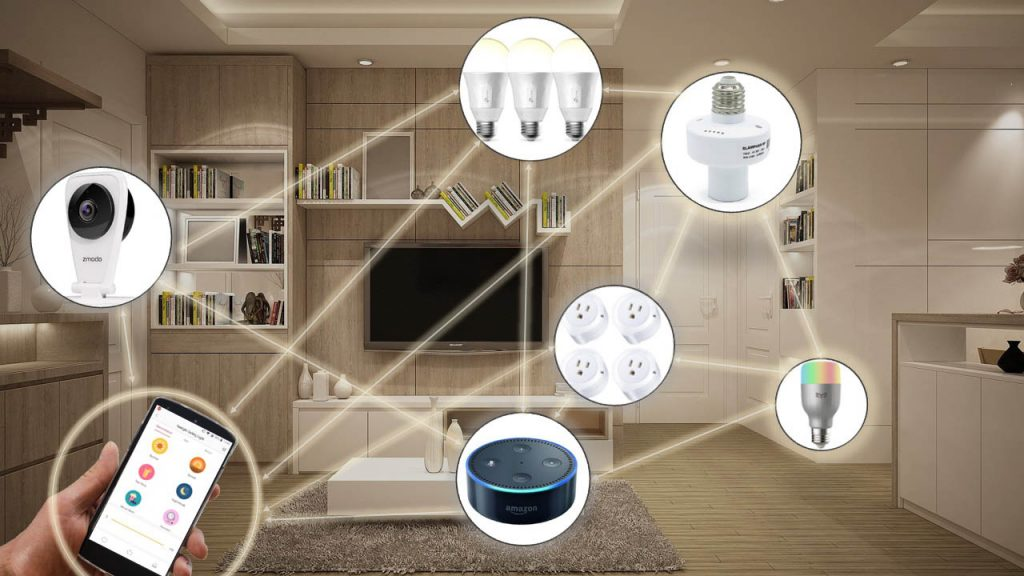
\includegraphics[width=0.6\columnwidth]{images/application_smart_home_1.jpg}
	\end{center}
	\caption{Dispositivi comunicano tra di loro nell'ecosistema casa}
	\label{fig:application_smart_home_1}
\end{figure}
\begin{figure}%
	\centering
	\subfloat[Google Home]{{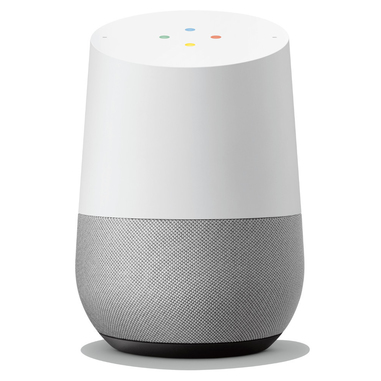
\includegraphics[width=4cm]{images/application_smart_home_2} }}%
	\qquad
	\subfloat[Google Nest]{{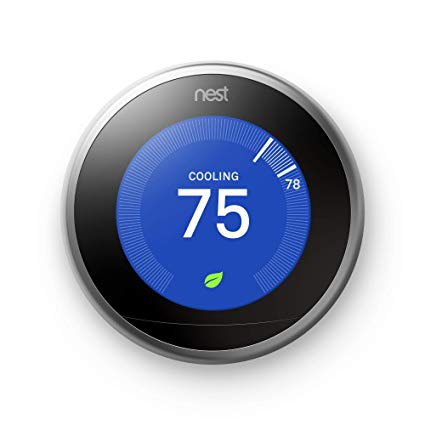
\includegraphics[width=4cm]{images/application_smart_home_3} }}%
	\caption{Esempi di soluzioni per l'ecosistema smart home}%
	\label{fig:application_smart_home_23}%
\end{figure}
In questo modo, dispositivi quali luci, termostati, sistemi di allarme possono essere attivati da remoto attraverso uno smartphone o attraverso un comando vocale o addirittura possono imparare le nostre abitudini, comunicare tra di loro, per decidere quali comportamenti intraprendere senza alcun intervento umano.


\subsection{Healthcare}
Uno degli ambiti nei quali il mondo dell'IoT potrebbe avere un impatto straordinario sulle persone è proprio quello dell'healthcare, rivoluzionando di fatto l'intera concezione legate a questo mondo.
Il fine delle applicazioni IoT in ambito medico è quello di migliorare la vita delle persone, migliorando e monitorando il loro stato di salute attraverso l'utilizzo di dispositivi indossabili ed interconnessi.
In questo modo, tali dispositivi avranno il compito di raccogliere dati che saranno fondamentali per una corretta creazione di un profilo dello stato di salute individuale e la conseguente creazione di piani personalizzati di cura.
\begin{figure}%
	\centering
	\subfloat[Adamm intelligent asthma management]{{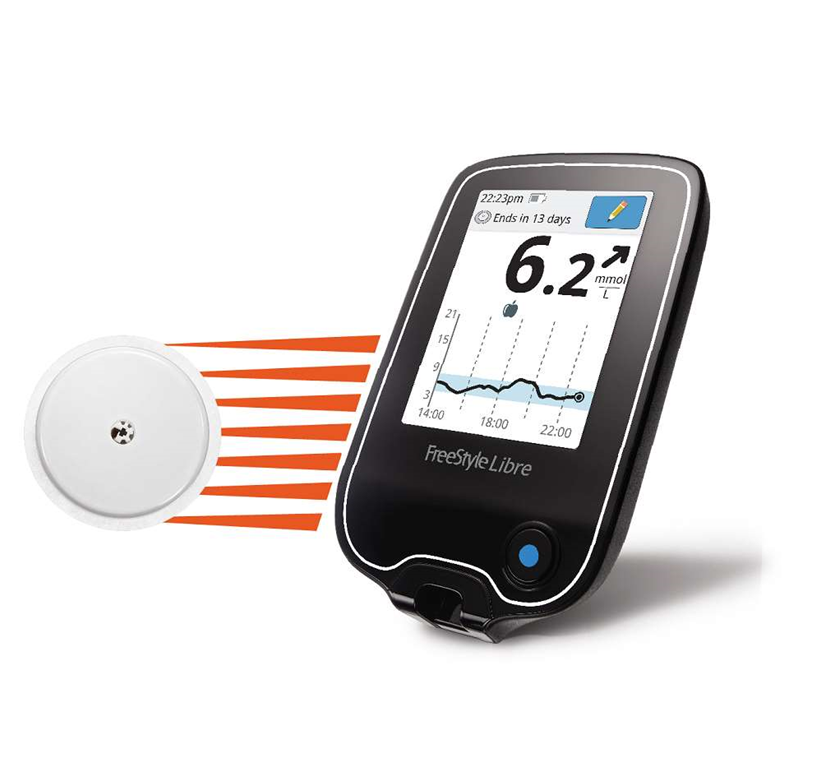
\includegraphics[width=6cm]{images/application_healthcare_1} }}%
	\qquad
	\subfloat[FreeStyle Libre Smart Glucometer]{{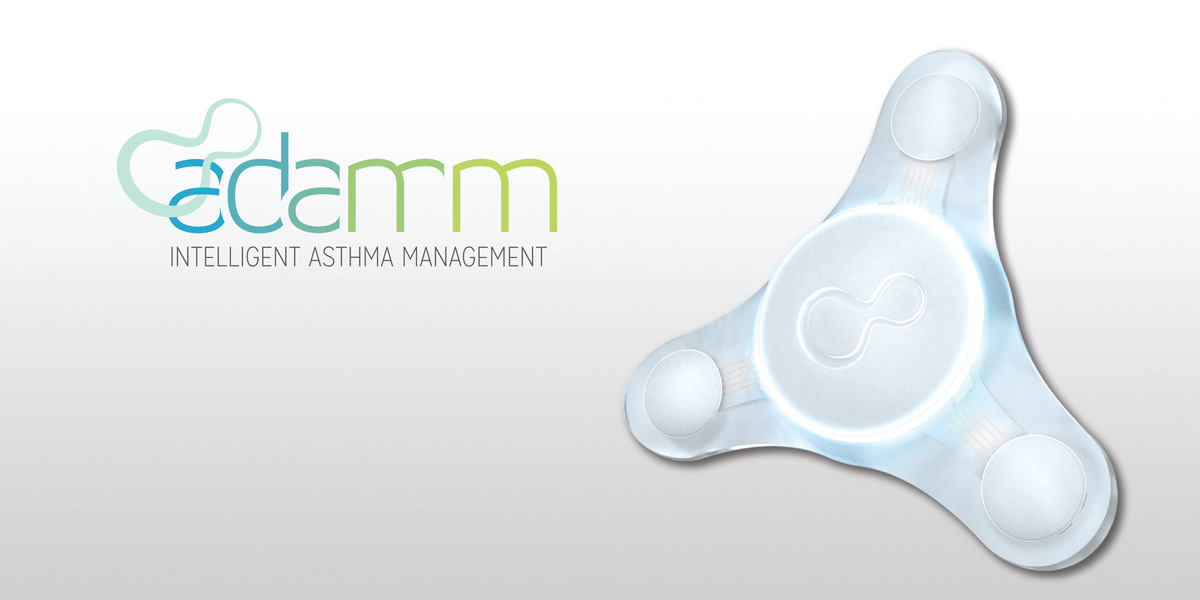
\includegraphics[width=6cm]{images/application_healthcare_2} }}%
	\caption{Soluzione per il monitoraggio dell'asma (sinistra) e per il monitoraggio del glucosio per pazienti affetti da diabete (destra)}%
	\label{fig:application_healthcare}%
\end{figure}

\subsection{Agriculture}
Data la continua crescita della popolazione mondiale, di pari passo incrementa anche la domanda di cibo e beni primari. Per fronteggiare a queste necessità, attraverso l'IoT è possibile dotare gli agricoltori di tecniche avanzate per incrementare la produzione e migliorare la qualità.
Gli agricoltori sono così in grado di raccogliere utili informazioni da sensori disposti nei campi che possano aiutarli nelle scalte da adottare nella coltivazione e controllare l'utilizzo di acqua e fertilizzanti.
\begin{figure}%
	\centering
	\subfloat{{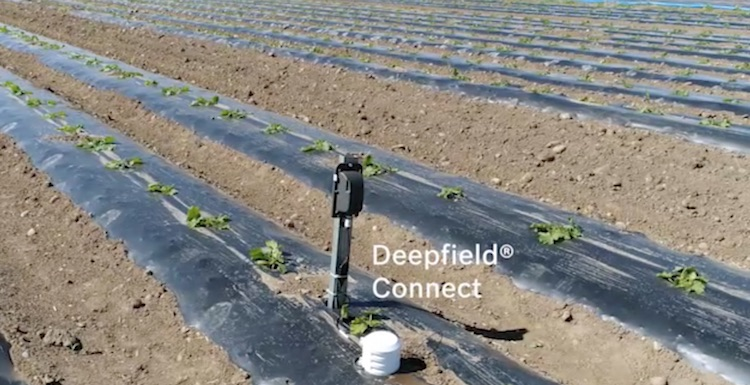
\includegraphics[width=6cm]{images/application_bosch_1} }}%
	\qquad
	\subfloat{{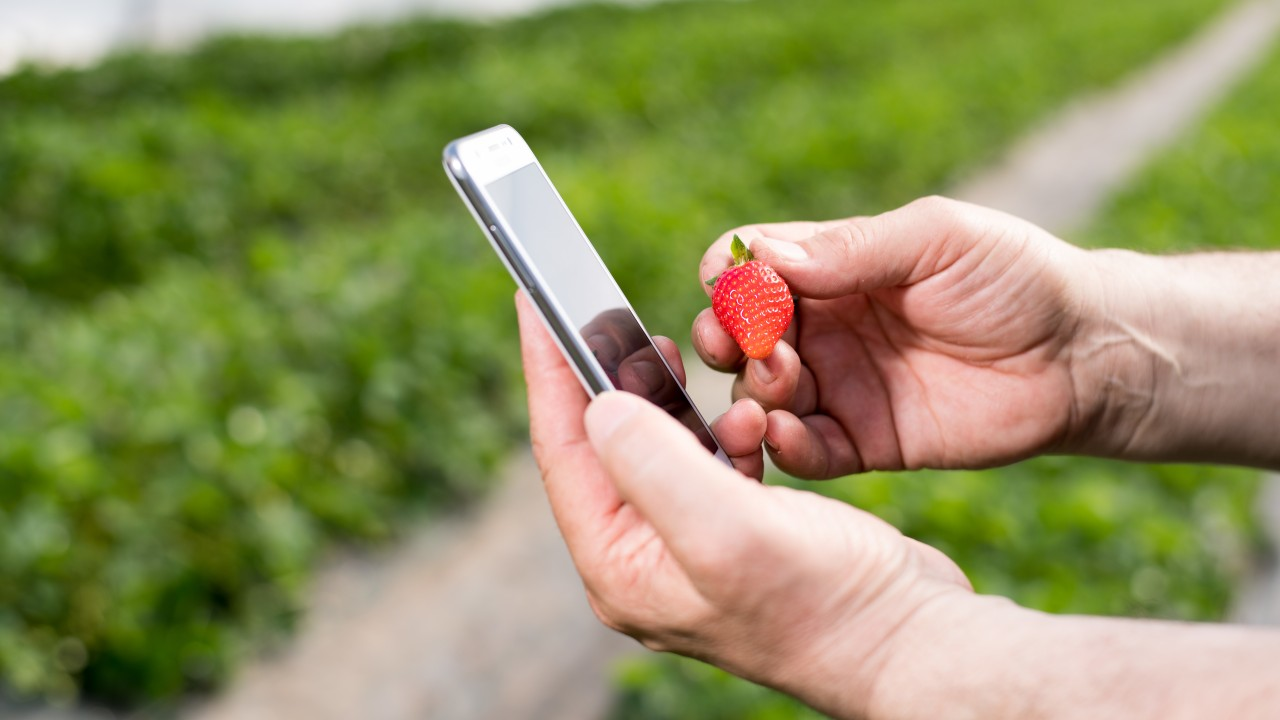
\includegraphics[width=6cm]{images/application_bosch_2} }}%
	\caption{Bosch Deepfield Connect Project}%
	\label{fig:application_bosch}%
\end{figure}
\subsection{Cities}
Il campo delle Smart Cities è talmente vasto ed offre talmente tanti spunti cha sarebbe riduttivo ricondurlo a pochi esempi applicativi. L'idea alla base dell'utilizzo di dispositivi IoT all'interno di una città è quello di automatizzare ed ottimizzare servizi quali i trasporti pubblici, inquinamento, sicurezza e regolamentare il traffico.
In questo modo, attraverso la distribuzione di una rete di sensori interconnessi tra loro, i cittadini possono essere in grado di trovare parcheggio, rilevare in anticipo ed eventualmente evitare aree trafficate, rilevare infrazioni e pericoli.
\subsection{Energy}
Il termine Smart Grid è diventato presto popolare in tutto il mondo, questo perchè il suo scopo è ambizioso ed è quello di raccogliere dati relativi alla richiesta e produzione energetica in maniera automatica, analizzare i comportamenti ed il consumo energetico per migliorare l'efficienza con la quale i fornitori distribuiscono l'energia e la rendono disponibile ai consumatori.
In questo modo è possibile ridurre i costi e l'impatto ambientale legati alla produzione dell'energia.
\begin{figure}
	\begin{center}
		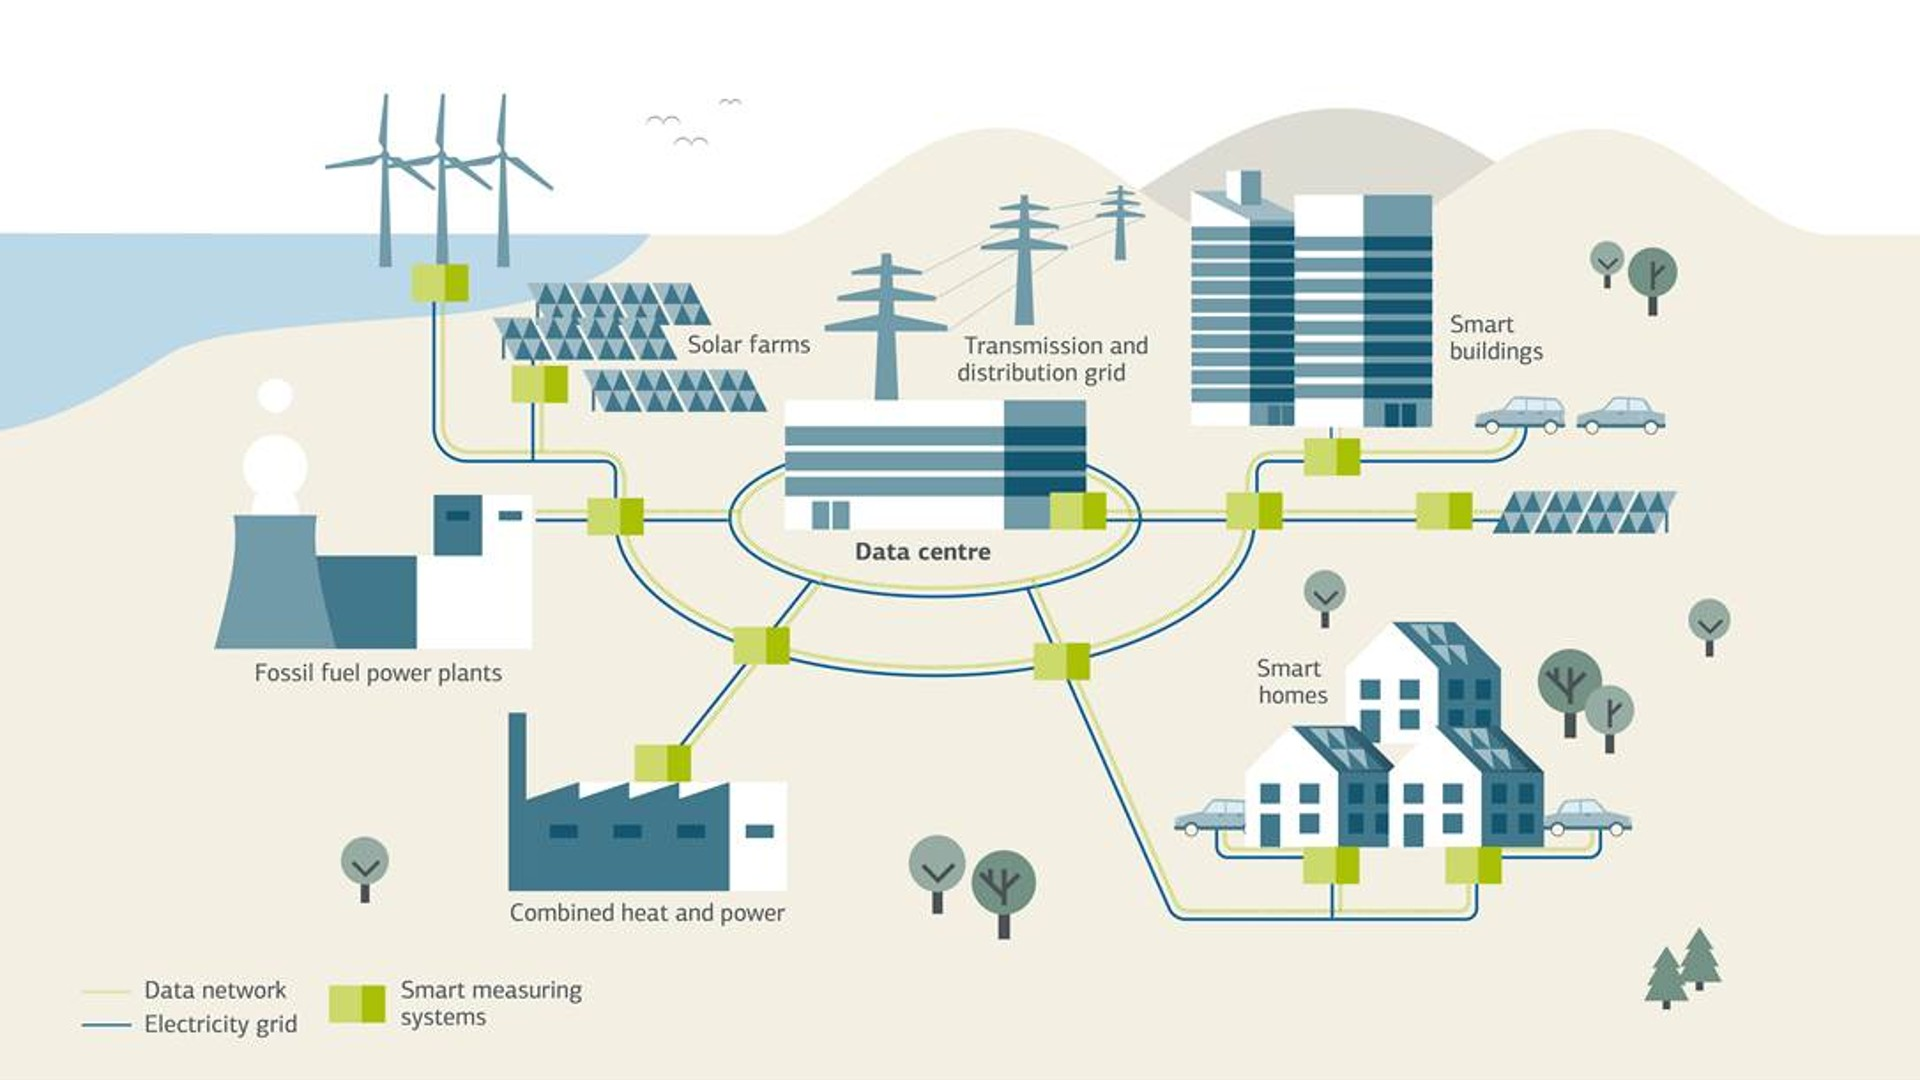
\includegraphics[width=0.8\columnwidth]{images/application_smart_grid_1}
	\end{center}
	\caption{Il concept delle smart grid}
	\label{fig:application_smart_grid_1}
\end{figure}
\subsection{Retail}
Il nostro modo di acquistare, scegliere e desiderare nuovi prodotti è stato già completamente rivoluzionato dalla possibilità di acquistare un capo di abbigliamento oppure l'ultima novità tecnologia oppure del pane fresco stando comodamente seduti in spiaggia o in ufficio e riceverlo entro poche ore.
Sono inoltre già presenti dispositivi IoT che effettuano ordini al nostro posto quando un certo prodotto si esaurisce o sta per farlo, in modo tale da non lasciarci mai senza. In questo modo, frigoriferi o dispense intelligenti acquistano per noi quello che ci serve.A questa rivoluzione del modo di comprare online che è già ampiamente consolidata, si sta avvicinando una nuova rivoluzione del modo di comprare anche dai negozi fisici. I negozi fisici infatti si trasformano e non hanno più casse dove pagare o commessi a rifornire gli scaffali, il tutto sostituto da una grande quantità di sensori, sistemi di visione ed in generale dispositivi IoT che sono in grado di capire cosa inseriamo nel nostro carrello, in quale quantità ed infine addebitare il tutto sul nostro smartphone senza alcuna cassa ne coda.
\begin{figure}
	\begin{center}
		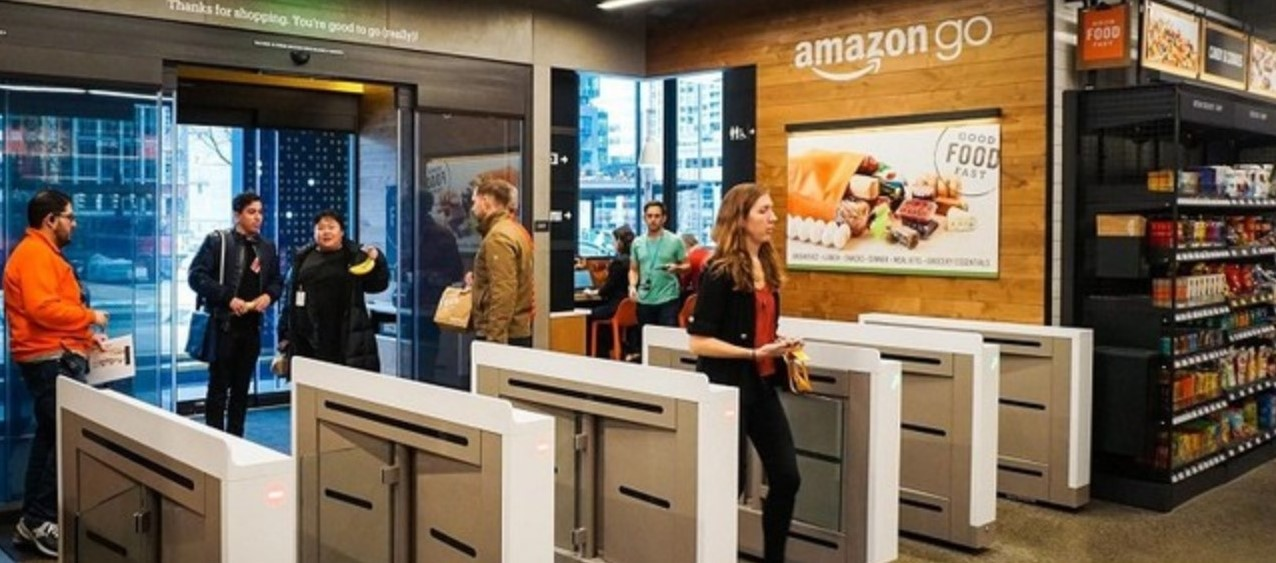
\includegraphics[width=0.8\columnwidth]{images/application_amazon_go}
	\end{center}
	\caption{Amazon Go store nella città di Seattle}
	\label{fig:application_amazon_go}
\end{figure}
In questa rivoluzione del modo di comprare e di vendere, gli smartphone sono il mezzo grazie al quale venditori e consumatori restano in contatto anche una volta fuori dal negozio. Inoltre essi, unitamente ad altri sensori e dispositivi interconnessi, rappresentano un modo per seguire i movimenti dei clienti all'interno dei negozi, in modo da poter addattare il layout dello store disponendo alcuni prodotti in zone a più elevato traffico.
\subsection{Automotive}
Nel campo della mobilità, l'IoT ha già offerto varie soluzioni finalizzate ad offrire al passeggero un maggiore confort, intrattenimento e sicurezza. Un esempio ne sono i consolidati sistemi di aiuto alla guida quali Cruise Control, Frenata Assistita, Rilevamento dei Pedoni, Rilevamento di Corsia etc. 
\begin{figure}
	\begin{center}
		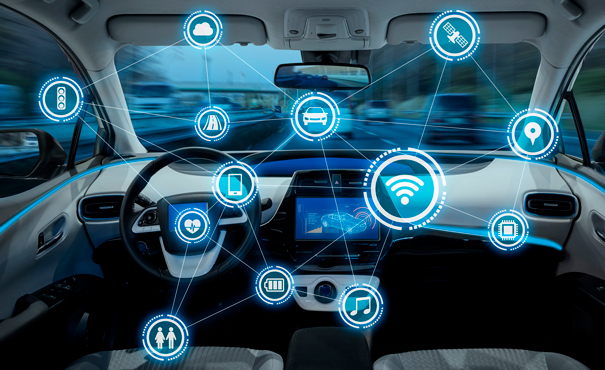
\includegraphics[width=0.8\columnwidth]{images/application_automotive}
	\end{center}
	\caption{The IoT Connected Car}
	\label{fig:application_automotive}
\end{figure}
Il prossimo step nella integrazione del mondo IoT con quello Automotive è quello di stabilire una comunicazione tra veicoli, finalizzata ad offrire nuovi servizi. Tale comunicazione potrà poi essere anche uno dei maggiori enabler per la guida autonoma di veicoli i quali, non soltanto saranno in grado di 'vedersi' ma anche di 'parlarsi'.\\
Questo è proprio il fulcro di questo lavoro di tesi che si concentrerà quindi sulla progettazione e prototipazione di un servizio IoT che, abilitando una comunicazione tra diversi veicoli, possa offrire ad ogni conducente un servizio in real time sul monitoraggio del traffico e, più in generale, di segnalazione di tutti gli eventi che potrebbero occorrere e potrebbero mettere a rischio la vita delle persone o anche soltanto che potrebbero consentire di raggiungere in un minor tempo la propria destinazione. Sarà infatti progettato e prototipato nei capitoli seguenti, un sistema di condivisione dei dati stradali attraverso una piattaforma di Crowdsourcing, termine che sarà spiegato nel dettaglio nel \autoref{chap:due}. Tali dati stradali, provenienti da diversi utenti, in diverse aree geografiche, potrenno essere poi obiettivo di una analisi dei dati con tecniche di Machine Learning per la scoperta di pattern, consigli sulla navigazione, sulla manutenzione ed ampiamento delle strade. Tale analisi di dati, sebbene nel \autoref{chap:due} e \autoref{chap:tre} venga sviluppata una interfaccia che renda possibile l'immediato utilizzo di tecniche di Machine Learning sui dati raccolti, sarà fuori dallo scopo di questo lavoro di tesi.










